% Problem 4.1: Non-uniform random numbers
% Notes and checklist: ../Exercises/4.01-non-uniform-random-numbers/README.md
% Figures:            \includegraphics{4.01-non-uniform-random-numbers/figures/<name>}
\exercise{1}{Non-uniform random numbers}

A computer only provides uniform random numbers $u \in [0,1)$. This problem turns them into
numbers with a prescribed density $f(x)$ ($f \ge 0$, $\int f = 1$) in two ways: by inverting the
cumulative distribution function (CDF) and by the hit-and-miss (rejection) method
\cite{Carlon2025}. All runs use \texttt{numpy.random.default\_rng} with seed~1.

\subsection{Inverse CDF method}

Let $F(x) = \int_{-\infty}^{x} f(y)\,dy$. Because $f \ge 0$, $F$ is non-decreasing, and where
$f > 0$ it is strictly increasing and invertible. If $u$ is uniform on $[0,1]$ and $y = F^{-1}(u)$, then
\begin{equation}
  P(y \le t) = P\big(F^{-1}(u) \le t\big) = P\big(u \le F(t)\big) = F(t),
\end{equation}
since $P(u \le a) = a$ for $a \in [0,1]$. The CDF of $y$ is therefore $F$, and its density is
$F'(t) = f(t)$.

The three requested densities have CDFs that can be inverted by hand:
\begin{align}
  f(x) &= \tfrac13 \text{ on } [-2,1]: & F(x) &= \tfrac{x+2}{3}, & x &= -2 + 3u, \\
  f(x) &= e^{-x} \text{ on } [0,\infty): & F(x) &= 1 - e^{-x}, & x &= -\ln(1-u), \\
  f(x) &= \tfrac{x+1}{2} \text{ on } [-1,1]: & F(x) &= \tfrac{(x+1)^2}{4}, & x &= 2\sqrt{u} - 1 .
\end{align}
We use $\ln(1-u)$ instead of $\ln u$, because $u = 0$ can occur and $1-u$ is never zero.
Figure~\ref{fig:4.1-inverse} shows that the histograms of $10^5$ numbers follow the exact densities
within the Poisson error bars $\sqrt{k}$ of a bin with $k$ entries.

\begin{figure}[htbp]
  \centering
  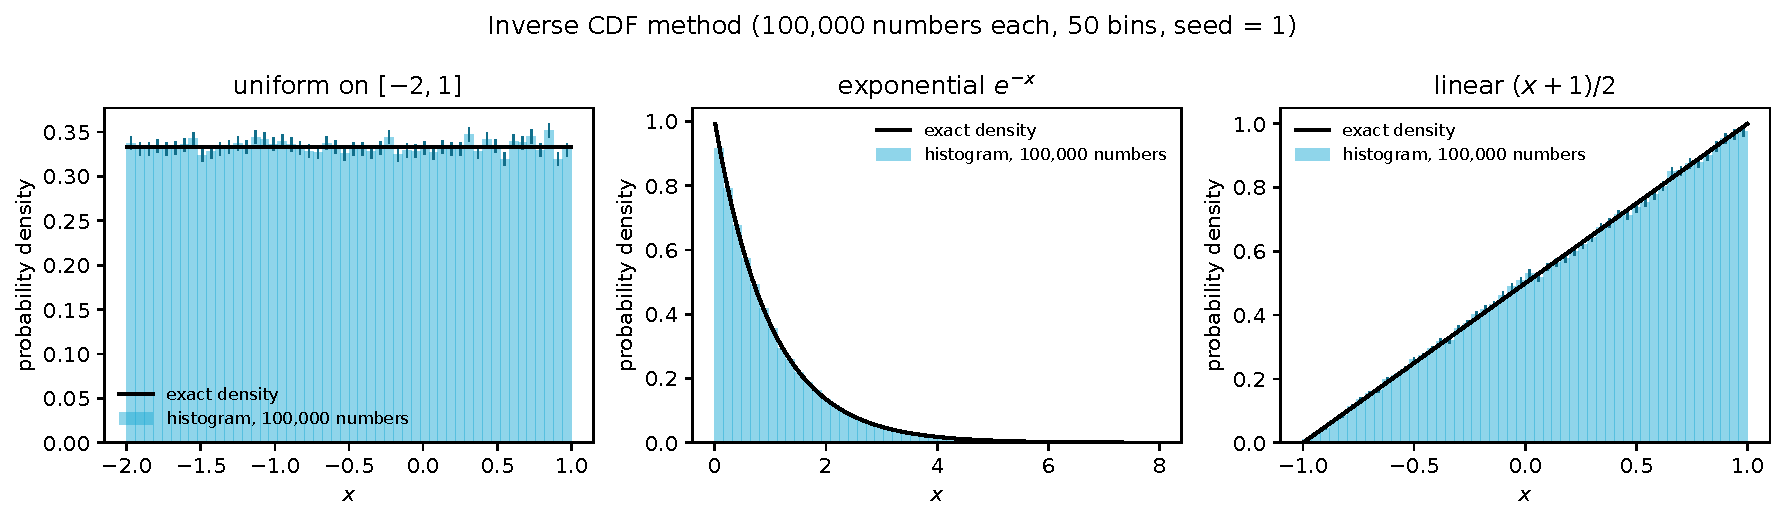
\includegraphics[width=\linewidth]{4.01-non-uniform-random-numbers/figures/a_inverse_cdf}
  \caption{Inverse CDF method: normalised histograms (50 bins, error bars $\sqrt{k}/(N\Delta x)$)
    of $N = 10^5$ numbers per density, with the exact density as a black line. Seed 1. The
    exponential histogram is cut at $x = 8$.}
  \label{fig:4.1-inverse}
\end{figure}

\subsection{Hit-and-miss method}

For $f$ supported on $[a,b]$ and bounded by $M$, we draw $t \sim U[a,b]$ and $s \sim U[0,M]$ and keep
$t$ if $s \le f(t)$. The pair $(t,s)$ is uniform in the box $[a,b]\times[0,M]$, so the kept points are
uniform in the region under the curve. The number of kept points near $t$ is proportional to the
height $f(t)$, so the kept $t$ have density $f$. This also works when $f$ is not normalised, because
only the shape of $f$ matters.

The fraction of kept points is the area under the curve divided by the area of the box,
\begin{equation}
  p_{\text{acc}} = \frac{\int_a^b f(x)\,dx}{M(b-a)} .
\end{equation}
For the linear density on $[-1,1]$ with $M = 1$ this is $1/2$. The second function,
$f(x) = -x(1-x)\,e^{-x^2}\ln(1-x)$ on $[0,1]$, is not normalised. Its maximum on a fine grid,
increased by 1\,\% to be safe, gives $M = 0.1582$, and numerical integration
(\texttt{scipy.integrate.quad}) gives $Z = \int_0^1 f = 0.09011$, so $p_{\text{acc}} = Z/M = 0.5697$.

\begin{table}[htbp]
  \centering
  \caption{Fraction of kept points in hit-and-miss, from $10^6$ tries each (seed 1). The error is
    the binomial standard error $\sqrt{p(1-p)/N_{\text{tries}}}$.}
  \label{tab:4.1-acceptance}
  \begin{tabular}{lccc}
    \toprule
    density & box & kept fraction & expected \\
    \midrule
    $(x+1)/2$ on $[-1,1]$                 & $[-1,1]\times[0,1]$      & $0.5007 \pm 0.0005$ & $0.5$ \\
    $-x(1-x)e^{-x^2}\ln(1-x)$ on $[0,1]$  & $[0,1]\times[0,0.1582]$  & $0.5705 \pm 0.0005$ & $0.5697$ \\
    unit disk (section~\ref{sec:4.1-disk}) & $[-1,1]^2$              & $0.7853 \pm 0.0004$ & $\pi/4 = 0.7854$ \\
    \bottomrule
  \end{tabular}
\end{table}

The measured fractions in table~\ref{tab:4.1-acceptance} agree with the prediction within 1.6
standard errors, and the histograms in figure~\ref{fig:4.1-hm} follow the (normalised) densities.
The method wastes the rejected points, so a box that fits $f$ tightly (small $M$) is more efficient.
A larger $M$ gives the same distribution, only at a lower acceptance rate.

\begin{figure}[htbp]
  \centering
  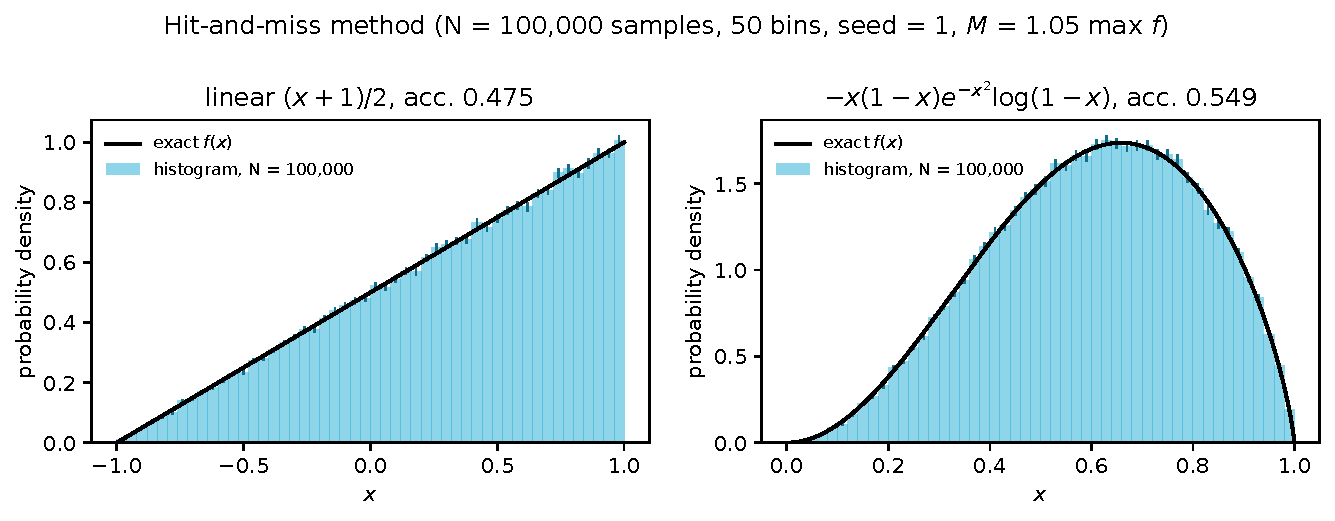
\includegraphics[width=0.9\linewidth]{4.01-non-uniform-random-numbers/figures/b_hit_and_miss}
  \caption{Hit-and-miss method with $10^6$ tries per density: histograms (50 bins) of the
    $500\,745$ and $570\,481$ kept numbers. The second density is divided by $Z = 0.09011$ to
    compare with the normalised histogram. Box heights $M = 1$ and $M = 0.1582$, seed 1.}
  \label{fig:4.1-hm}
\end{figure}

\subsection{Uniform points in a disk with hit-and-miss}
\label{sec:4.1-disk}

Points $(x,y)$ uniform in the square $[-1,1]^2$ are kept when $x^2 + y^2 \le 1$. The kept points are
uniform in the unit disk (figure~\ref{fig:4.1-disk}, left). The kept fraction is the area ratio
$\pi/4$, which gives a Monte Carlo estimate of $\pi$ as a by-product:
\begin{equation}
  \pi \approx 4 \times 0.7853 = 3.1410 \pm 0.0016 .
\end{equation}

\subsection{Uniform points in a disk in polar coordinates}

A uniform density on the unit disk is $1/\pi$ per unit area. With the area element
$dA = r\,dr\,d\theta$ this becomes
\begin{equation}
  f(r,\theta)\,dr\,d\theta = \frac{1}{\pi}\, r\,dr\,d\theta
  = \underbrace{2r\,dr}_{r \in [0,1]} \; \underbrace{\frac{d\theta}{2\pi}}_{\theta \in [0,2\pi)} .
\end{equation}
The density factorises, so $r$ and $\theta$ are independent. The angle is uniform,
$\theta = 2\pi v$, and the radius has $F(r) = r^2$, so the inverse CDF method of the first subsection gives
$r = \sqrt{u}$, with $u$ and $v$ two independent uniform numbers. No point is rejected.

\kulbox[5pt]{Uniform points in the unit disk without rejection: $\theta = 2\pi v$ and $r = \sqrt{u}$.
The square root comes from the Jacobian $r$ of the polar coordinates.}

The naive choice $r = u$ gives a flat radial density instead of $2r$: the same number of points
lands in every ring, while the area of a ring grows with $r$. The points then pile up near the centre
(figure~\ref{fig:4.1-disk}, right). Figure~\ref{fig:4.1-radial} confirms that both correct methods give
the radial density $2r$, and that $r = u$ does not.

\begin{figure}[htbp]
  \centering
  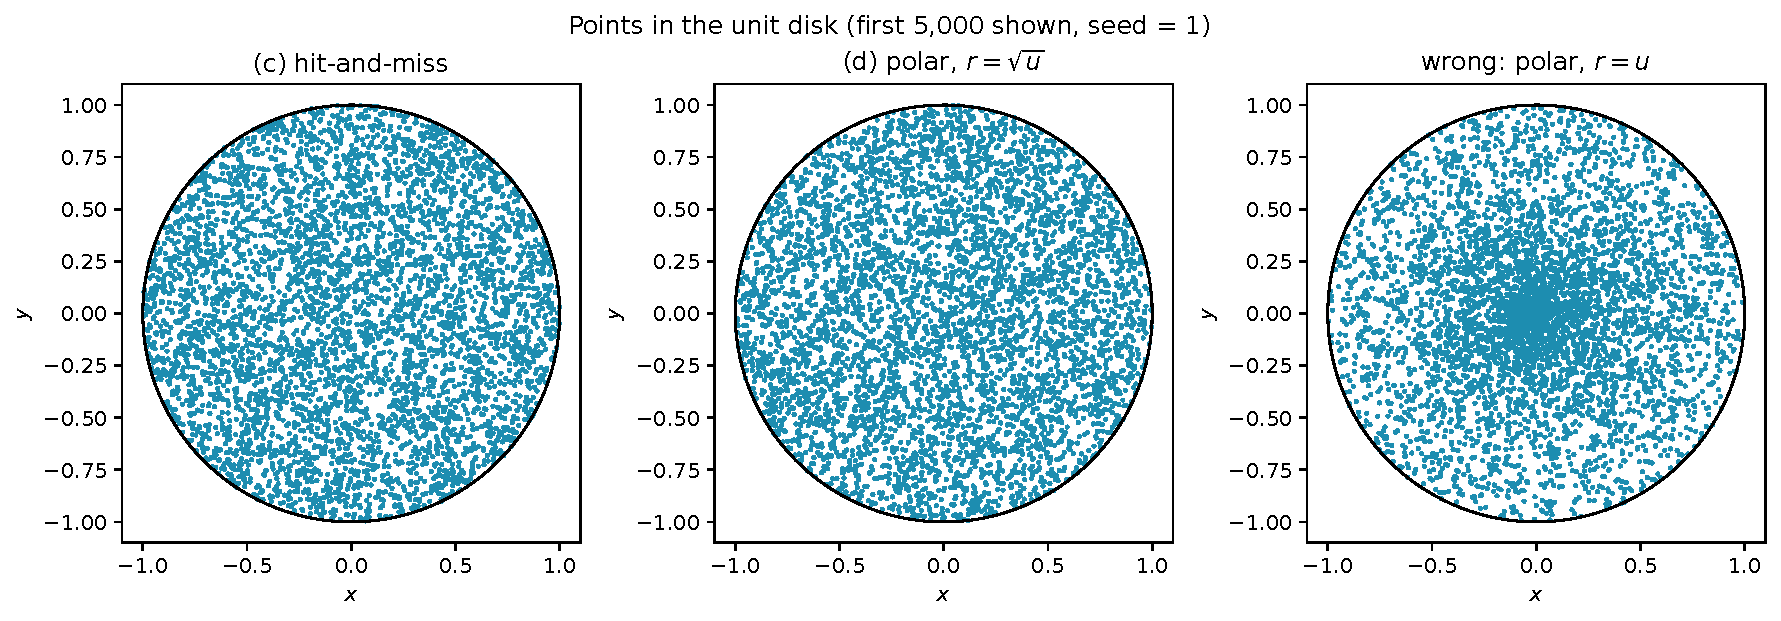
\includegraphics[width=\linewidth]{4.01-non-uniform-random-numbers/figures/cd_disk_scatter}
  \caption{Points in the unit disk (the first 5\,000 shown). Left: hit-and-miss in $[-1,1]^2$,
    $10^6$ tries. Middle: polar coordinates with $r = \sqrt{u}$, $N = 10^5$. Right: the wrong choice
    $r = u$, $N = 10^5$, which crowds the centre. Seed 1.}
  \label{fig:4.1-disk}
\end{figure}

\begin{figure}[htbp]
  \centering
  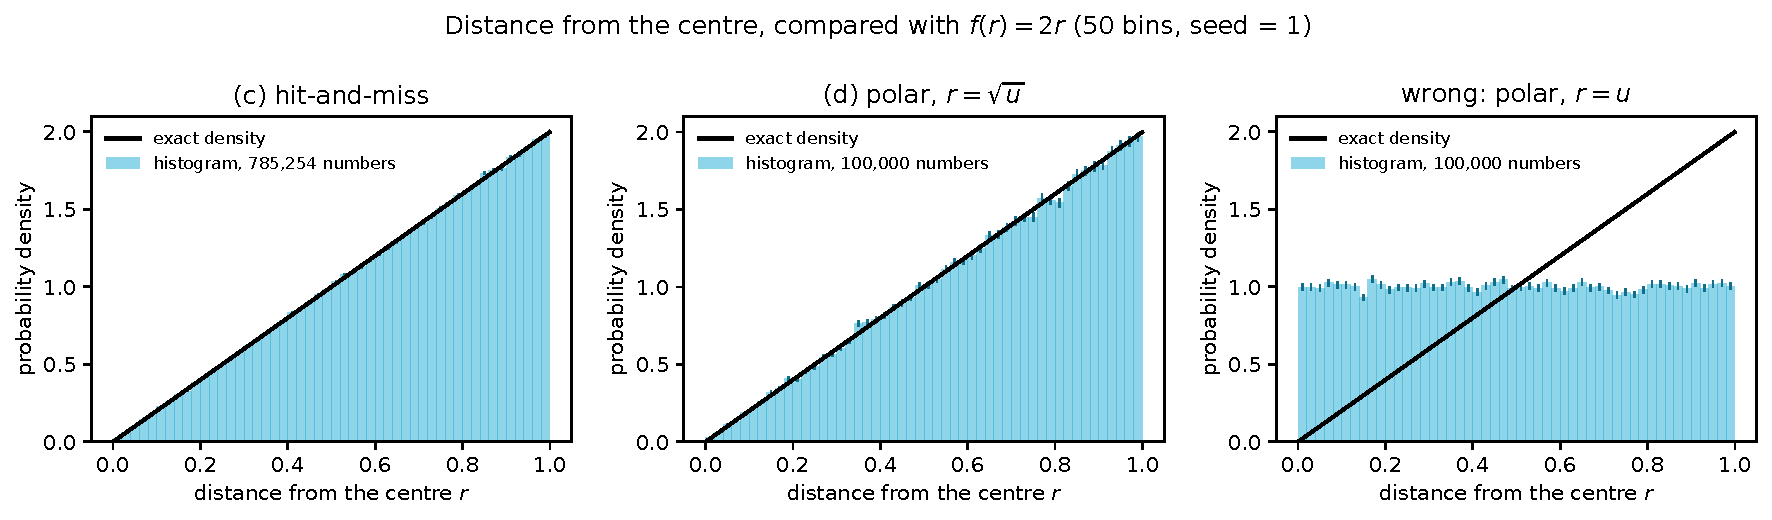
\includegraphics[width=\linewidth]{4.01-non-uniform-random-numbers/figures/cd_radial_density}
  \caption{Histograms (50 bins) of the distance $r$ to the centre for the three samples of
    figure~\ref{fig:4.1-disk} ($785\,254$ kept hit-and-miss points, $10^5$ polar points each),
    compared with the density $f(r) = 2r$ of a uniform disk. Seed 1.}
  \label{fig:4.1-radial}
\end{figure}
